%%%%%%%%%%%%%%%%%%%%%%%%%%%%%%%%%%%%%%%%%%%%%%%%%%%%%%%%%%%%%%%%%%%%%%%%%%%%%%%%
%%
%% Uppsala Beamer theme example by Frédéric Haziza <daz@it.uu.se>
%%
%% Describing beamerthemeUppsala version 2008/05/15
%%
%% If you have more than three sections or more than three subsections in at least
%% one section, you might want to use the [hideallsubsections] or
%% [hideothersubsections] switch.  In this case, only the current (sub-) section is
%% displayed in the sidebar and not the full overview.
%%
%% Options are:
%% ===========
%% * hideallsubsections, hideothersubsections
%% * nonumbers,totalnumber
%% * withnav, mylogo
%% * grey
%% * noprogressbar
%%
%% For the sidebar layout:
%% * subsectionsattop, sectionpathattop
%% 
%% Removed
%% =======
%% * sidebarshades
%%
%% Tip
%% ===
%% latex this file to see the theme in action
%%
%%%%%%%%%%%%%%%%%%%%%%%%%%%%%%%%%%%%%%%%%%%%%%%%%%%%%%%%%%%%%%%%%%%%%%%%%%%%%%%%

\documentclass{beamer}
%\documentclass[handout]{beamer}
%\documentclass[notes]{beamer}
%\documentclass[trans]{beamer}

\usetheme[hideothersubsections]{Uppsala}
\usepackage{hyperref}
%\hypersetup{
%    colorlinks=true,
%    filecolor=blue,      
%    urlcolor=blue,
%    citecolor=cyan,
%}
\usepackage{graphicx}
\usepackage{geometry}
\usepackage{subfigure}
\usepackage{color}
\usepackage{wrapfig}
\usepackage{graphicx}
\usepackage{graphics}
\usepackage{graphfig}
\usepackage{xcolor}
\usepackage{amsmath}
\usepackage{wrapfig}
\usepackage{geometry}
\usepackage{subfigure}
\usepackage{float}
\usepackage{wrapfig}
\usepackage{graphics}
\usepackage{graphfig}
\usepackage{xcolor}
\usepackage{listings}
\usepackage{indentfirst}
\usepackage{hyperref}
\usepackage{pgf}
\usepackage{tikz}
\usepgflibrary{arrows}
\usepgflibrary{shapes}
\usetikzlibrary{%
  arrows,%
  calc,%
  fit,%
  patterns,%
  plotmarks,%
  shapes.geometric,%
  shapes.misc,%
  shapes.symbols,%
  shapes.arrows,%
  shapes.callouts,%
  shapes.multipart,%
  shapes.gates.logic.US,%
  shapes.gates.logic.IEC,%
  er,%
  automata,%
  backgrounds,%
  chains,%
  topaths,%
  trees,%
  petri,%
  mindmap,%
  matrix,%
  calendar,%
  folding,%
  fadings,%
  through,%
  positioning,%
  scopes,%
  decorations.fractals,%
  decorations.shapes,%
  decorations.text,%
  decorations.pathmorphing,%
  decorations.pathreplacing,%
  decorations.footprints,%
  decorations.markings,%
  shadows}

\usepackage[english]{babel} % or whatever
\usepackage[utf8]{inputenc} % or whatever
\usepackage{mathptmx}
\usepackage{helvet}
%\usepackage{courier}
\usepackage{xcolor}

\usepackage[T1]{fontenc}
% Or whatever. Note that the encoding and the font should match. If T1
% does not look nice, try deleting the line with the fontenc.

%% -----------------------------------------------------------
%% MISC. INFORMATION
%% -----------------------------------------------------------

\title{ \emph{Properties of Penalized Least Squares Estimator(PLSE)}}
\subtitle{}

\author[Zhiyang Liang \emph{}] % appears in the footline
{Zhiyang Liang}

\institute[School of Data Science] % appears in the footline
{
  School of Data Science\\
  Fudan University
}

\date[December 13] % appears in the bottom of the sidebar
{December 13,\ 2021}

%% \logo{...}

%% This is only inserted into the PDF information catalog. Can be left out.
%\subject{Unofficial Beamer Theme for Uppsala University}

%% -----------------------------------------------------------
%% Extra ``local'' settings
%% -----------------------------------------------------------

% Comment out this, if you do not want the table of contents to pop up at
% the beginning of each (sub)section:
\AtBeginSection[]
{
  \begin{frame}<beamer> % with <beamer> => doesn't appear in handout mode
    \frametitle{Outline} %% Put the title you want, or none!
    \tableofcontents[currentsection,currentsubsection]
    %\tableofcontents[currentsection]
  \end{frame}
}

%% Unfolds piecewise element with shading.
%% Text appears, shaded, and the audience knows that something is coming
%% Note: if you set the number too high, the audience will try to read the 
%% text that now shows up more, and will be disturbed.
%% ``dynamic'' makes elements show gradually more and more.
\setbeamercovered{transparent=5}
%% \setbeamercovered{dynamic=5}

%% -----------------------------------------------------------

\begin{document}

\newcommand{\SubItem}[1]{
    {\setlength\itemindent{15pt} \item[-] #1}
}

\begin{frame}[plain] %% Gets the frame to fill up the page, no menu/sidebar/footline
  \titlepage
\end{frame}

\begin{frame}
    \frametitle{Outline}
    \tableofcontents[currentsection]
\end{frame}
%%%%%%%%%%%%%%%%%%%%%%%%%%%%%%%%%%%%%%%%%%%%%%%%%%%%%%%%%%%%%%%%%%%%%%%%%%%%%%%%% Introduction
\section{Review of The Last Lecture}
\begin{frame}
	\frametitle{Review of The Last Lecture}
Fan and Li (2001) advocate penalty functions that give estimators with the following three properties:
  \begin{enumerate}
  	\item \emph{Sparsity} : The resulting estimator sets small estimate coefficients to zero.
  	\item \emph{Unbiasedness} : The resulting estimator is nearly unbiased, especially when the true $\beta_j$ is large.
  	\item \emph{Continuity} : The resulting estimator is continuous in the data to reduce instability in model prediction (Breiman,1996).

  \end{enumerate}
\end{frame}
%%%%%%%%%%%%%%%%%%%%%%%%%%%%%%%%%%%%%%%%%%%%%%%%%%%%%%%%%%%%%%%%%%%%%%%%%%%%%%%%% Introduction
\begin{frame}
	\frametitle{Review of The Last Lecture}
	Let $p_\lambda(\theta)$ be nondecreasing and continuously differentiable on $\left [ 0,\infty \right ) $. Assume that the function 
	$-\theta -p'_\lambda(\theta)$ is strictly unimodal on $\left ( 0,\infty \right ) $ with the convention $p'_\lambda(0) = p'_\lambda(0+)$. 
	\begin{enumerate}
		\item \emph{Sparsity} : if $\min_{\theta\geq 0 }\{\theta+p'_\lambda(\theta)\} > 0$, which holds if $p'_\lambda(0+) > 0$;
		\item \emph{Approximate Unbiasedness} : if $p'_\lambda(\theta) =0 $ for large $\theta$;
		\item \emph{Continuity} : if and only if $arg\min_{\theta\geq 0}\{\theta+p'_\lambda(\theta)\} = 0$.
  
	\end{enumerate}
\end{frame}
%%%%%%%%%%%%%%%%%%%%%%%%%%%%%%%%%%%%%%%%%%%%%%%%%%%%%%%%%%%%%%%%%%%%%%%%%%%%%%%%%
\begin{frame}
  \frametitle{Examples of Nonconcave Penalties}
  \begin{figure}[h]
    \centering
    \subfigure{
      \begin{minipage}[t]{0.5\linewidth}
        \centering
        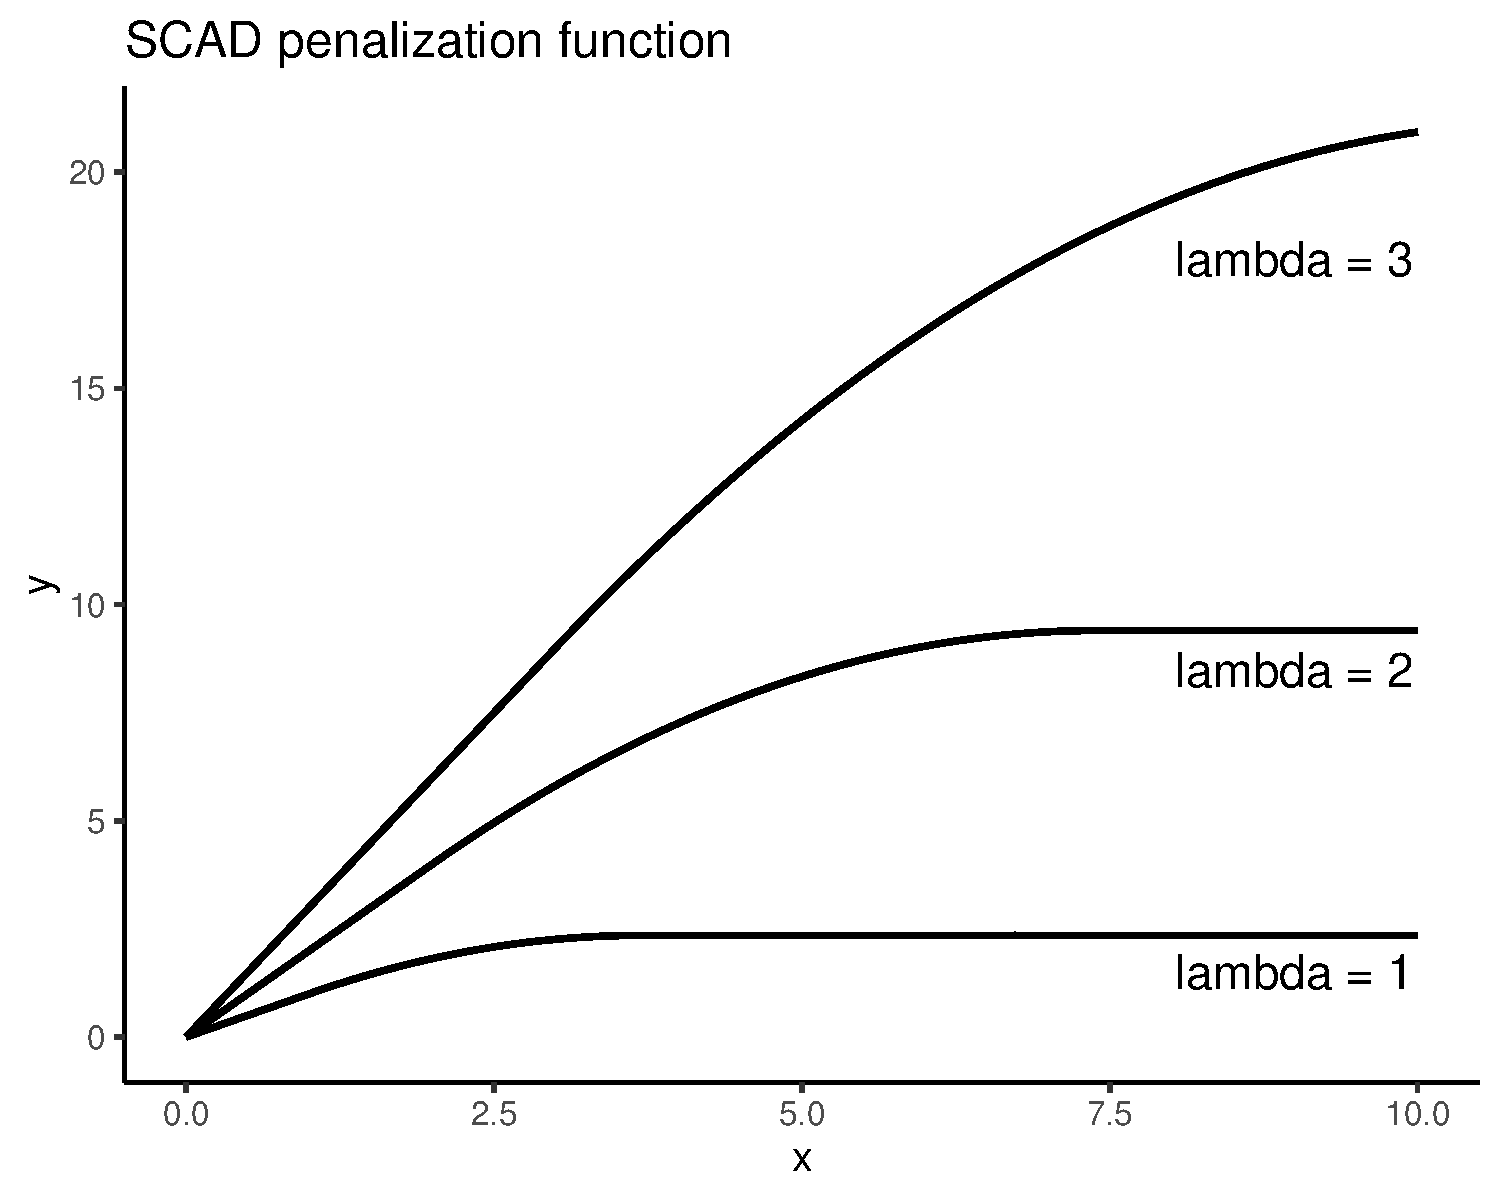
\includegraphics[scale=0.2]{scad.pdf}
        %\caption{m = 1}
      \end{minipage}%
    }%
    \subfigure{
      \begin{minipage}[t]{0.5\linewidth}
        \centering
        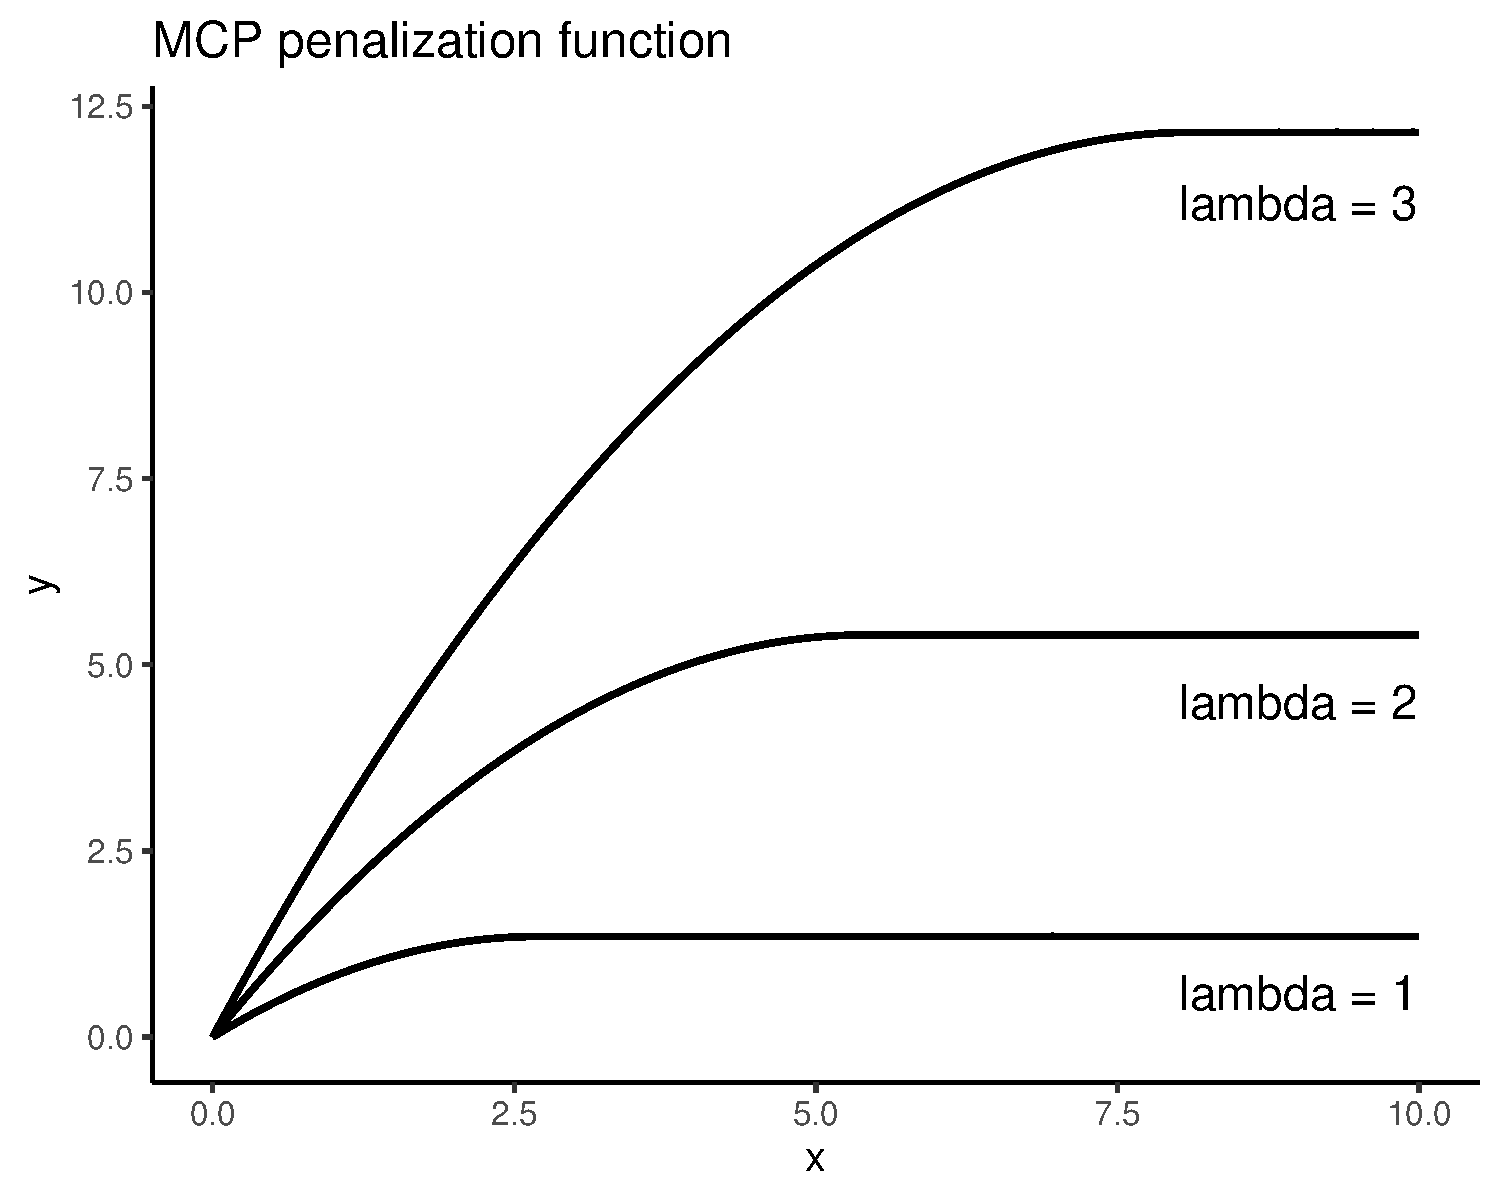
\includegraphics[scale=0.2]{mcp.pdf}
        %\caption{m = 2}
      \end{minipage}
    }
    \centering
    \caption{Plot of SCAD and MCP penalization functions for different values of parameters $\lambda$, with $a = 2.7$ for MCP and $a = 3.7$ for SCAD.}\label{scad_mcp}
  \end{figure}
\end{frame}
%%%%%%%%%%%%%%%%%%%%%%%%%%%%%%%%%%%%%%%%%%%%%%%%%%%%%%%%%%%%%%%%%%%%%%%%%%%%%%%%% Graph Deviation Networks
\section{Proof in Orthonormal Case}
\begin{frame}
	\frametitle{Proof in Orthonormal Case}
	In the orthonormal case, we can consider the following penalized least squares problem:Minimize with
	repect to $\theta$
	\[\ell(\theta) = (z-\theta)^2/2 + p_\lambda(|\theta|)\]

\end{frame}
%%%%%%%%%%%%%%%%%%%%%%%%%%%%%%%%%%%%%%%%%%%%%%%%%%%%%%%%%%%%%%%%%%%%%%%%%%%%%%%%%
\begin{frame}
	\frametitle{Theoretical Results}
	\begin{enumerate}
    \item The solution exists and is unique.
		\item The solution satisfies
		\[\hat{\theta}(z)=\left\{\begin{array}{ll}
			0 & \text { if }|z| \leq p_{0} \\
			z-\operatorname{sgn}(z) p_{\lambda}^{\prime}(|\hat{\theta}(z)|) & \text { if }|z|>p_{0}
			\end{array}\right.\]
		where $p_0 = \min_{\theta \geq 0}\{\theta + p'_\lambda(\theta)\}$. Moreover, $|\hat \theta(z)|\leq|z|$.
    \item If $p'_\lambda(\cdot)$ is nonincreasing, the for $|z| > p_0$, we have 
    \[|z|-p_{0} \leq|\hat{\theta}(z)| \leq|z|-p_{\lambda}^{\prime}(|z|) \]
    \item When $p'_\lambda(\theta)$ is continuous on $\left(0,\infty \right)$, the solution $\hat \theta(z)$
    is continuous if and only if the minimum of $|\theta|+p'_\lambda(|\theta|)$ is attained at point zero.
    
	\end{enumerate}
\end{frame}
%%%%%%%%%%%%%%%%%%%%%%%%%%%%%%%%%%%%%%%%%%%%%%%%%%%%%%%%%%%%%%%%%%%%%%%%%%%%%%%%%
\begin{frame}
	\frametitle{Result 1 and 2}
  When $z = 0$, it is clear that
  $\hat \theta(z) = 0$ is the unique minimizer.
  ~\\
  Without loss of generality, assume
  that $ z > 0$. Then, for all $\theta > 0$, $\ell(-\theta)>\ell(\theta)$. Hence, $\hat \theta(z) \geq 0 $. Note
  that for $\theta> 0$,
  \[\ell'(\theta) = \theta -z +p'_\lambda(\theta)\]
  When $z < p_0$, the function $\ell$ is strictly increasing on $\left( 0,\infty \right )$ because
the derivative function is positive. Hence, $\hat \theta(z)=0$. 
\end{frame}
%%%%%%%%%%%%%%%%%%%%%%%%%%%%%%%%%%%%%%%%%%%%%%%%%%%%%%%%%%%%%%%%%%%%%%%%%%%%%%%%%
\begin{frame}
	\frametitle{Result 1 and 2}
  When the function
$\ell'(\theta)$ is strictly increasing, there is at most one zero-crossing,
and hence the solution is unique.
Thus, we only need to consider the
case that $\ell'(\theta)$ has a valley on $\left( 0,\infty \right )$ and $z > p_0$. In this case, there
are two possible zero-crossings for the function $\ell'$ on $\left( 0,\infty \right )$. The
larger one is the minimizer because the derivative function at that
point is increasing. Hence, the solution is unique and satisfies
\begin{equation}
\hat{\theta}(z)=z-p_{\lambda}^{\prime}(\hat{\theta}(z)) \leq z 
\label{center}
\end{equation}
Thus, $\hat{\theta}(z) \leq z-p_{\lambda}^{\prime}(z) $ when $p_{\lambda}^{\prime}(\cdot) $ is nonincreasing. 
\end{frame}
%%%%%%%%%%%%%%%%%%%%%%%%%%%%%%%%%%%%%%%%%%%%%%%%%%%%%%%%%%%%%%%%%%%%%%%%%%%%%%%%%
\begin{frame}
  \frametitle{Result 3}
  Let $\theta_0$ be the
minimizer of $\theta+p_{\lambda}^{\prime}(\theta) $ over $[0, \infty)$. Then, from the preceding argument,
$\hat{\theta}(z)>\theta_{0} $ for $z > p_0$. If $p_{\lambda}^{\prime}(\cdot) $ is nonincreasing, then
\[ p_{\lambda}^{\prime}(\hat{\theta}(z)) \leq p_{\lambda}^{\prime}\left(\theta_{0}\right) \leq \theta_{0}+p_{\lambda}^{\prime}\left(\theta_{0}\right)=p_{0} \]
Since we have (\ref{center}), the result 3 holds.
\end{frame}
%%%%%%%%%%%%%%%%%%%%%%%%%%%%%%%%%%%%%%%%%%%%%%%%%%%%%%%%%%%%%%%%%%%%%%%%%%%%%%%%%
\begin{frame}
  \frametitle{Result 4}
  It is clear that continuity of the solution $\hat{\theta}(z)$ at the point $ z=p_{0} $
  if and only if the minimum of the function $|\theta|+p_{\lambda}^{\prime}(|\theta|)$ is attained at $0$.
  ~\\
  ~\\
  The continuity at other locations follows directly from the monotonicity and continuity of the function 
  $\theta+   p_{\lambda}^{\prime}(\theta)$  in the interval  $(0, \infty)$ .
\end{frame}
%%%%%%%%%%%%%%%%%%%%%%%%%%%%%%%%%%%%%%%%%%%%%%%%%%%%%%%%%%%%%%%%%%%%%%%%%%%%%%%%%
\section{Conclusion}
\begin{frame}
  \frametitle{Conclusion}
  When  $p_{\lambda}^{\prime}(0+)>0$, $p_{0}>0 $. Thus, for $ |z| \leq p_{0}$ , 
  the estimator is thresholded to $0$ . 

  ~\\
  For  $|z|>p_{0}$ , the solution has a shrinkage property. 

  ~\\
  And if $|z| \rightarrow+\infty $, $p_{\lambda}^{\prime}(|z|) \rightarrow 0 $ then $\hat \theta(z) \approx z$, since (\ref{center}) holds. 
\end{frame}
%%%%%%%%%%%%%%%%%%%%%%%%%%%%%%%%%%%%%%%%%%%%%%%%%%%%%%%%%%%%%%%%%%%%%%%%%%%%%%%%%
%%%%%%%%%%%%%%%%%%%%%%%%%%%%%%%%%%%%%%%%%%%%%%%%%%%%%%%%%%%%%%%%%%%%%%%%%%%%%%%%%
%%%%%%%%%%%%%%%%%%%%%%%%%%%%%%%%%%%%%%%%%%%%%%%%%%%%%%%%%%%%%%%%%%%%%%%%%%%%%%%%%
\begin{frame}
\centering
\Huge{\textbf{ THANKS} }
\end{frame}
%%%%%%%%%%%%%%%%%%%%%%%%%%%%%%%%%%%%%%%%%%%%%%%%%%%%%%%%%%%%%%%%%%%%%%%%%%%%%%%%%
\end{document}
